\chapter{Sampling Methods}
\label{chap:sm}

\section{Inverse transform sampling}
\label{sec:sm:inverse_transform}
 inverse transform sampling. 

In the one-dimensional case, this amounts to converting a uniform random variable (which are easy to generate) into a variable sampled from a general distribution $f(\theta)$. One first finds its cumulative distribution function (CDF):
\begin{equation}
  F(\theta) = \int\limits_{-\infty}^\theta f(\theta^\prime) d\theta^\prime,
\end{equation}
computes the inverse of the CDF, and then applies this function to a uniform random variable  $x\sim U(0,1)$ to generate a variable $\theta = F^{-1}(x)$, which is distributed according to $f(\theta)$. 

In the general $D$-dimensional case, one calculates $D$ conditional distributions $\{f_i:i=1\ldots,D\}$: by marginalising over parameters with indices greater than $i$ and conditioning on parameters with indices less than $i$:
%
\begin{equation}
  f_i(\theta_i|\theta_{i-1},\ldots,\theta_1) 
  =
  \frac{%
    \int f_i(\params) d\theta_{i+1}\ldots d\theta_{N}
  }{%
    \int f_i(\params) d\theta_{i}\ldots d\theta_{N}
  },
\end{equation}
%
Integrating these yields $D$ conditional CDFs:
%
\begin{equation}
  x_i = F_i(\theta_i|\theta_{i-1},\ldots,\theta_1) = \int\limits_0^{\theta_i} f_i(\theta_i^\prime|\theta_{i-1},\ldots,\theta_1) d\theta_i^\prime.
\end{equation}
%
Inverting this gives $\theta_i = F^{-1}_i(x_i|\theta_{i-1},\ldots,\theta_1)$, which constitutes a set of relations sequentially transforming $D$ uniform random variables $\{x_i\}$ into $\{\theta_i\}$ distributed according to $f(\params)$.

In many cases, the prior $\prior(\params)$ is separable, and the above equations are easily calculated. For sections of the parameters which are not separable, the calculation can become more involved. We include a few demonstrations of this procedure in Section~\ref{sec:bay:prior_tranformations}. 



\section{Rejection Sampling}
\label{sec:sm:rejection}

\section{Importance Sampling}
\label{sec:sm:importance}

\section{Metropolis Methods}
\label{sec:sm:mh}

\section{Slice sampling}
\label{sec:sm:slice}
Radford Neal initially proposed slice sampling as an effective methodology for generating samples numerically from a given posterior $\posterior(\params)$. One first chooses a `slice' (or probability level) $\posterior_0$ uniformly within $[0,\posterior_\smax]$. One then samples uniformly within the $\params$-region defined by $\posterior(\params)>\posterior_0$. The similarity with the iso-likelihood contour sampling required by nested sampling should be clear. In the one-dimensional case, he suggests the sampling procedure detailed in Figure~\ref{fig:bay:1d_slice}.

\begin{figure}
  \centerline{%
    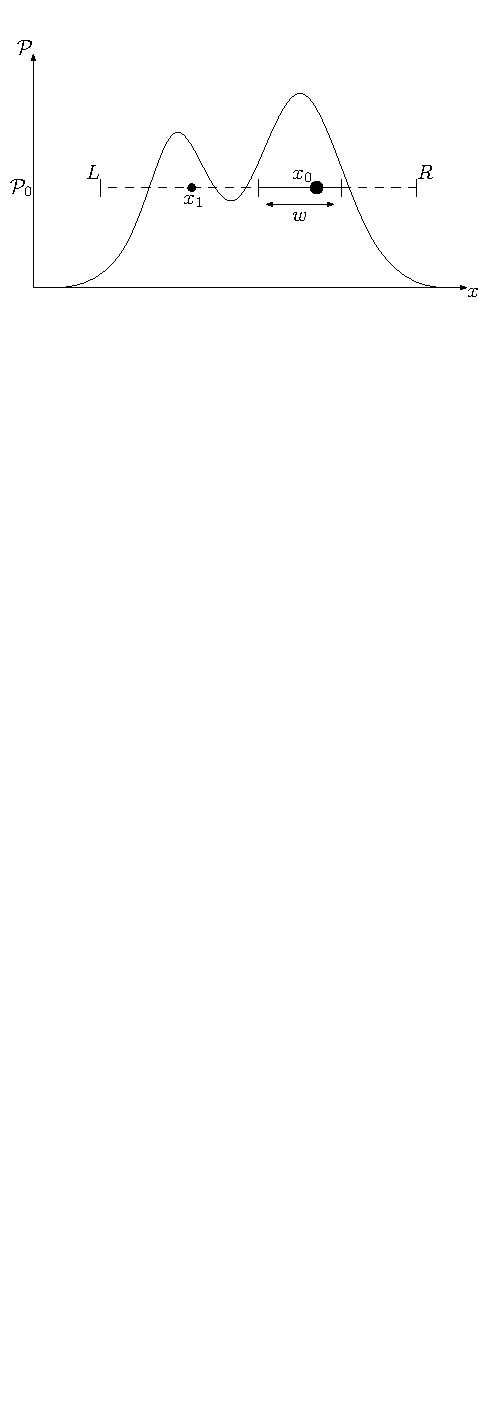
\includegraphics[width=\textwidth]{slice}
  }

  \caption{Slice sampling in one dimension. 
    Given a probability level (or slice) $\posterior_0$, slice sampling samples within the horizontal region defined by $\posterior>\posterior_0$. 
    From an initial point $x_0$ within the slice ($\posterior(x_0)>\posterior_0$), a new point $x_1$ is generated within the slice with a distribution $P(x_1|x_0)$.
    External bounds are first set on the slice $\hat{L}<x_0<\hat{R}$ by uniformly expanding a random initial bound of width $w$ until they lie outside the slice (Neal terms this the {\em stepping out\/} procedure). 
    $x_1$ is then sampled uniformly within these bounds.  
    If $x_1$ is not in the slice, then $\hat{L}$ or $\hat{R}$ is replaced with $x_1$, ensuring that $x_0$ is still within the slice.
    This procedure is guaranteed to generate a new point $x_1$, and satisfies detailed balance $P(x_0|x_1) = P(x_1|x_0)$. Thus, if $x_0$ is drawn from a uniform distribution within the slice, so is $x_1$.\label{fig:bay:1d_slice}
  }
\end{figure}



In higher dimensions,~\cite{NealSlice} suggests a variety of MCMC-like methods. The simplest of these is implemented by sampling each of the parameter directions in turn. Since each one-dimensional slice requires $\bigO{\text{a few}}$ likelihood calculations, the number of likelihood calculations required scales linearly with dimensionality, providing the region is efficiently navigated. Multi-dimensional slice sampling has many of the benefits of a traditional MH approach, and uses a proposal distribution which is much more efficient at sampling a hard likelihood constraint.
